\subsection{SGX Software Attestation}
\label{sec:sgx_attestation}

The software attestation scheme implemented by SGX follows the principles
outlined in \S~\ref{sec:generic_software_attestation}. An SGX-enabled processor
computes a measurement of the code and data that is loaded in each enclave,
which is similar to the measurement computed by the TPM~(\S~\ref{sec:tpm}). The
software inside an enclave can start a process that results in an SGX
attestation signature, which includes the enclave's measurement and an enclave
message.

\begin{figure}[hbt]
  \centering
  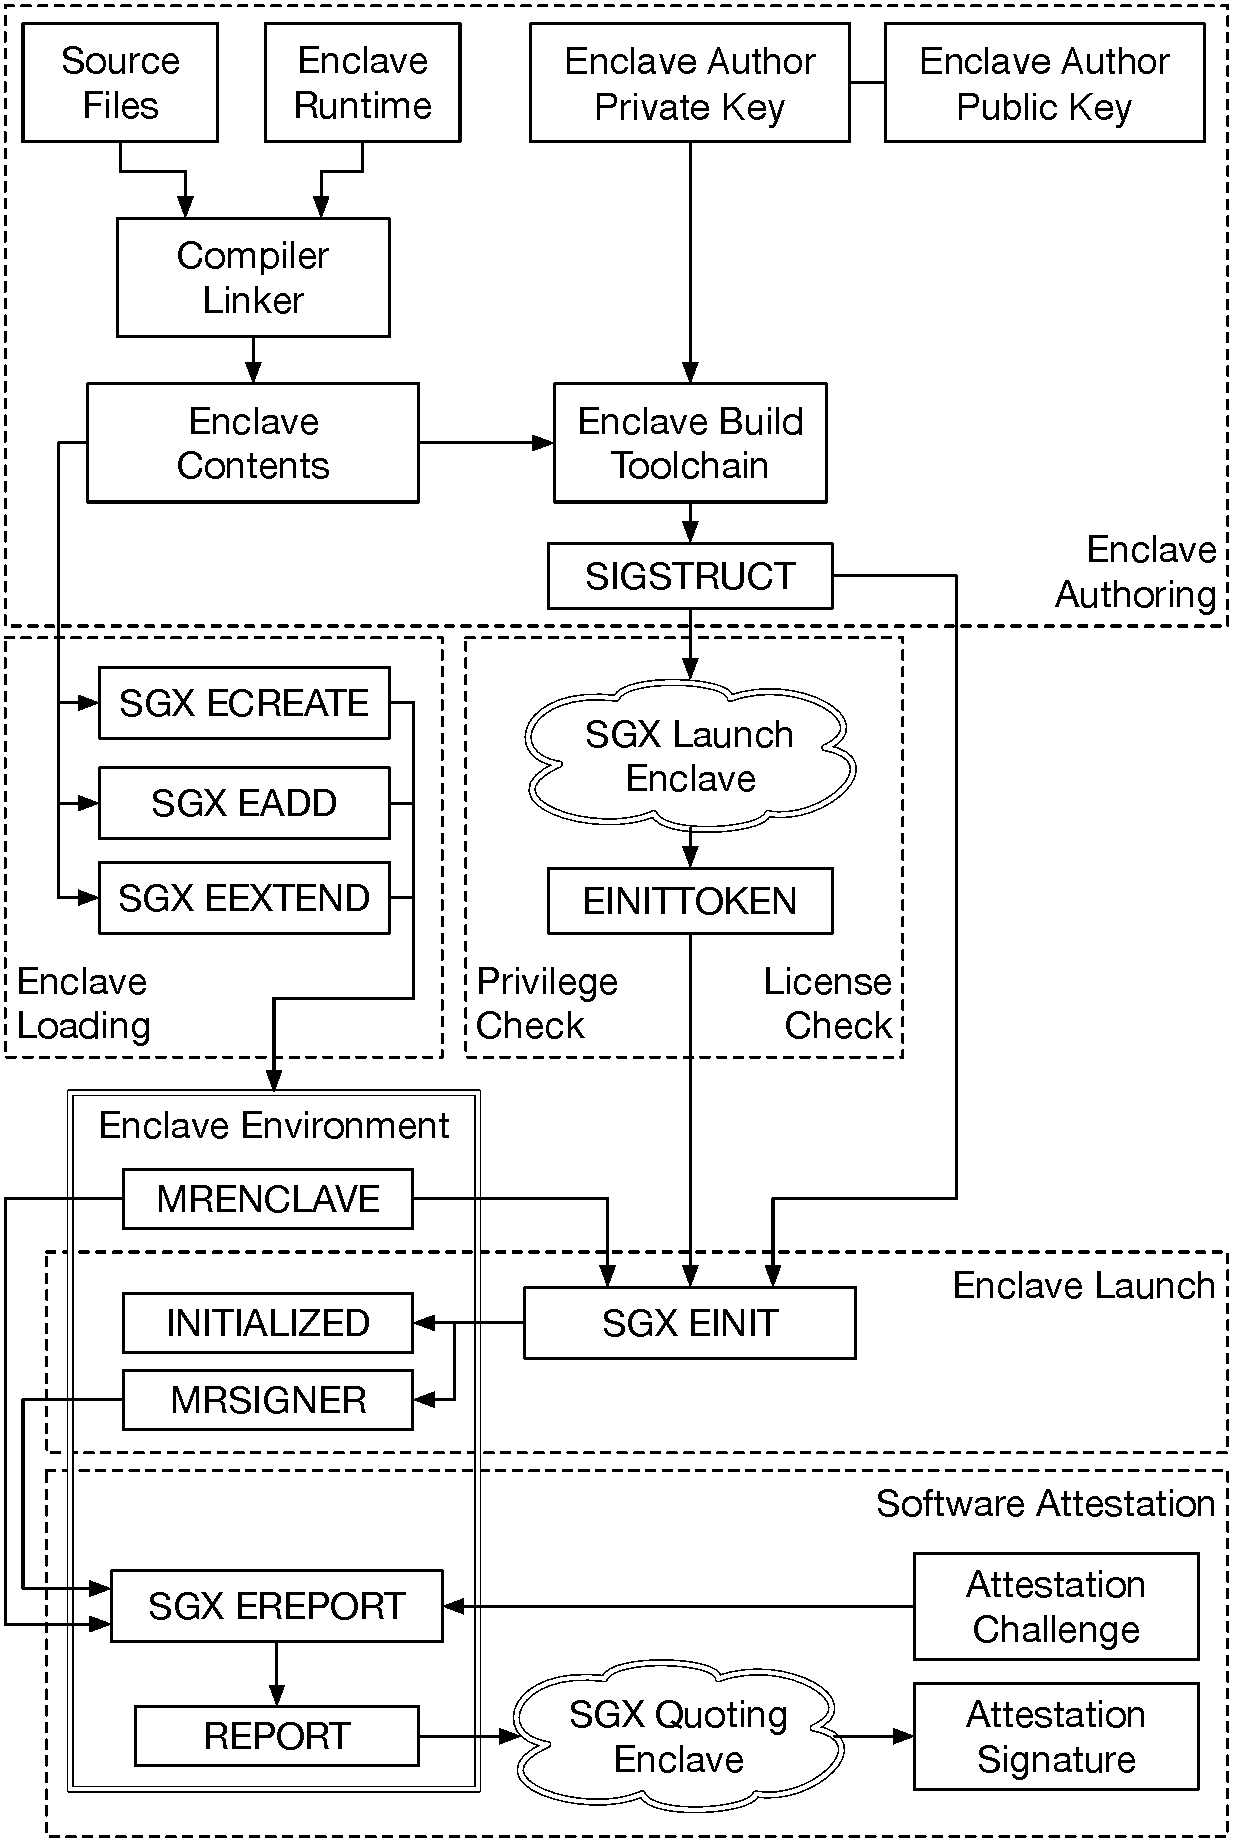
\includegraphics[width=85mm]{figures/sgx_attestation_overview.pdf}
  \caption{
    Setting up an SGX enclave and undergoing the software attestation process
    involves the SGX instructions \texttt{EINIT} and \texttt{EREPORT}, and two
    special enclaves authored by Intel, the SGX Launch Enclave and the SGX
    Quoting Enclave.
  }
  \label{fig:sgx_attestation_overview}
\end{figure}

% EPID signing takes too long for microcode.
%   US 8,972,746 B2 - 33:16-29, 33:58

The cryptographic primitive used in SGX's attestation signature is too complex
to be implemented in hardware, so signing process is performed by a privileged
\textit{Quoting Enclave}, which is issued by Intel, and can access the SGX
attestation key. This enclave is discused in \S~\ref{sec:sgx_quoting_enclave}.

Pushing the signing functionality into the Quoting Enclave creates the need for
a secure communication path between an enclave that desires to undergo
software attestation and the Quoting Enclave. The SGX design solves this
problem with a local attestation mechanism that can be used by an enclave to
prove its identity to any other enclave hosted by the same SGX-enabled CPU.
This scheme, described in \S~\ref{sec:sgx_ereport}, is implemented by the
\texttt{EREPORT} instruction.

% Keys: SDM S 39.4.3
% ISCA SGX Slides 104, 105, 106

The SGX attestation key used by the Quoting Enclave does not exist at the time
SGX-enabled processors leave the factory. The attestation key is provisioned
later, using a largely undocumented process that is known to involve at least
one other enclave issued by Intel, and at least two special \texttt{EGETKEY}
key types. The publicly available details of this process are summarized in
\S~\ref{sec:sgx_quoting_enclave}.

The SGX implementation contained in a CPU's hardware does not directly enforce
the enclave attribute checks that decide which enclaves can access the CPU
secrets used for software attestation. The potentially complex restrictions on
enclave attributes are instead enforced by the \textit{Launch Enclave}, which
is an enclave issued by Intel that gets to approve every other enclave before
it is initialized by \textit{EINIT}~(\S~\ref{sec:sgx_einit_overview}). The
officially documented information about the approval process is discussed in
\S~\ref{sec:sgx_launch_enclave}.

% Enclave License
%   US 8,972,746 B2 - 34:6-23
% Licenses are evaluated into Permits (which became EINITTTOKEN)
%   US 8,972,746 B2 - 34:24-29, 35:27-59
% EINIT requires a Permit to launch a production enclave
%   US 8,972,746 B2 - 35:60-67, 36:1-3, 36:47-52, 38:4-65
% License Enclave creates Permit
%   US 8,972,746 B2 - 36:40-46, 37:50-67, 38:1-3
% EMKPERMIT seems to have gotten merged into EINIT
%   US 8,972,746 B2 - 36:53-67, 37:1-7, 37:24-49
% License became SIGSTRUCT
%   US 8,972,746 B2 - 37:8-23

One of the SGX patents~\cite{intel2013patent1} discloses in no uncertain terms
that the Launch Enclave was introduced to ensure that each enclave's author has
a business relationship with Intel, and implements a software licensing system.
\S~\ref{sec:sgx_licensing} briefly discusses the implications, should this turn
out to be true.


\subsubsection{Local Attestation}
\label{sec:sgx_ereport}

% Using REPORTs for Local Attestation: SDM S 39.4.3.2
% EREPORT: SDM S 41.4.1

An enclave proves its identity to another \textit{target enclave} via the
\texttt{EREPORT} instruction shown in Figure~\ref{fig:sgx_ereport}. The SGX
instruction produces an attestation \textit{Report} (REPORT) that
cryptographically binds a message supplied by the enclave with the enclave's
measurement-based~(\S~\ref{sec:sgx_measurement}) and
certificate-based~(\S~\ref{sec:sgx_certificate_identity}) identities. The
cryptographic binding is accomplished by a MAC tag computed using a symmetric
key that is only shared between the target enclave and the SGX implementation.

\begin{figure}[hbt]
  \centering
  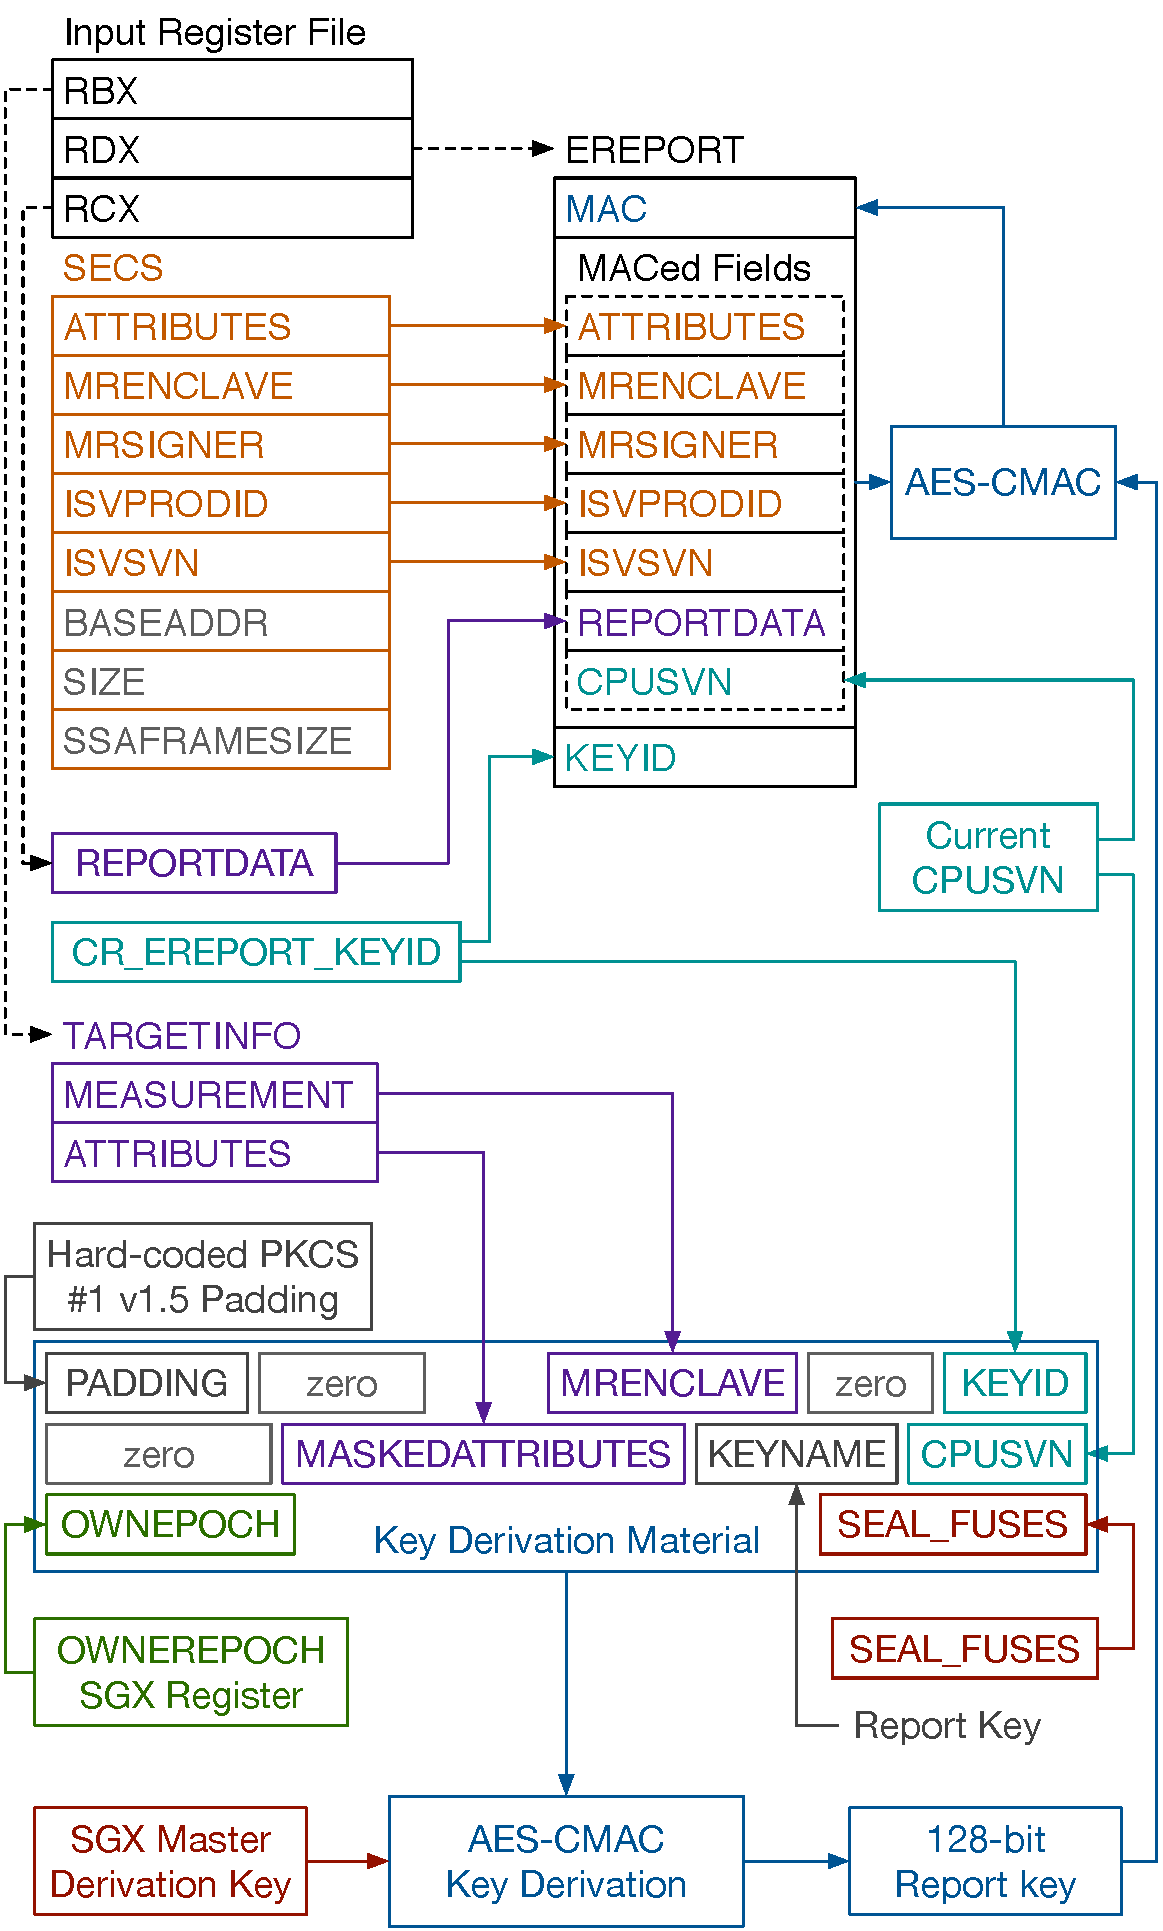
\includegraphics[width=85mm]{figures/sgx_ereport.pdf}
  \caption{
    \texttt{EREPORT} data flow
  }
  \label{fig:sgx_ereport}
\end{figure}

The \texttt{EREPORT} instruction reads the current enclave's identity
information from the enclave's SECS~(\S~\ref{sec:sgx_secs}), and uses it to
populate the REPORT structure. Specifically, \texttt{EREPORT} copies the
SECS fields indicating the enclave's measurement (MRENCLAVE), certificate-based
identity (MRSIGNER, ISVPROD, ISVSVN), and attributes (ATTRIBUTES). The
attestation report also includes the SVN of the SGX implementation (CPUSVN)
and a 64-byte (512-bit) message supplied by the enclave.

% Keys: SDM S 39.4.3

The target enclave that receives the attestation report can convince itself of
the report's authenticy as shown in Figure~\ref{fig:sgx_ereport_check}. The
report's authenticity proof is its MAC tag. The key required to verify the MAC
can only be obtained by the target enclave, by asking
\texttt{EGETKEY}~(\S~\ref{sec:sgx_egetkey}) to derive report key. The SDM
states that the MAC tag is computed using a block cipher-based
MAC~(CMAC,~\cite{fips2005cmac}), but stops short of specifying the underlying
cipher. One of the SGX papers~\cite{anati2013sgx} states that the CMAC is based
on 128-bit AES.


\begin{figure}[hbt]
  \centering
  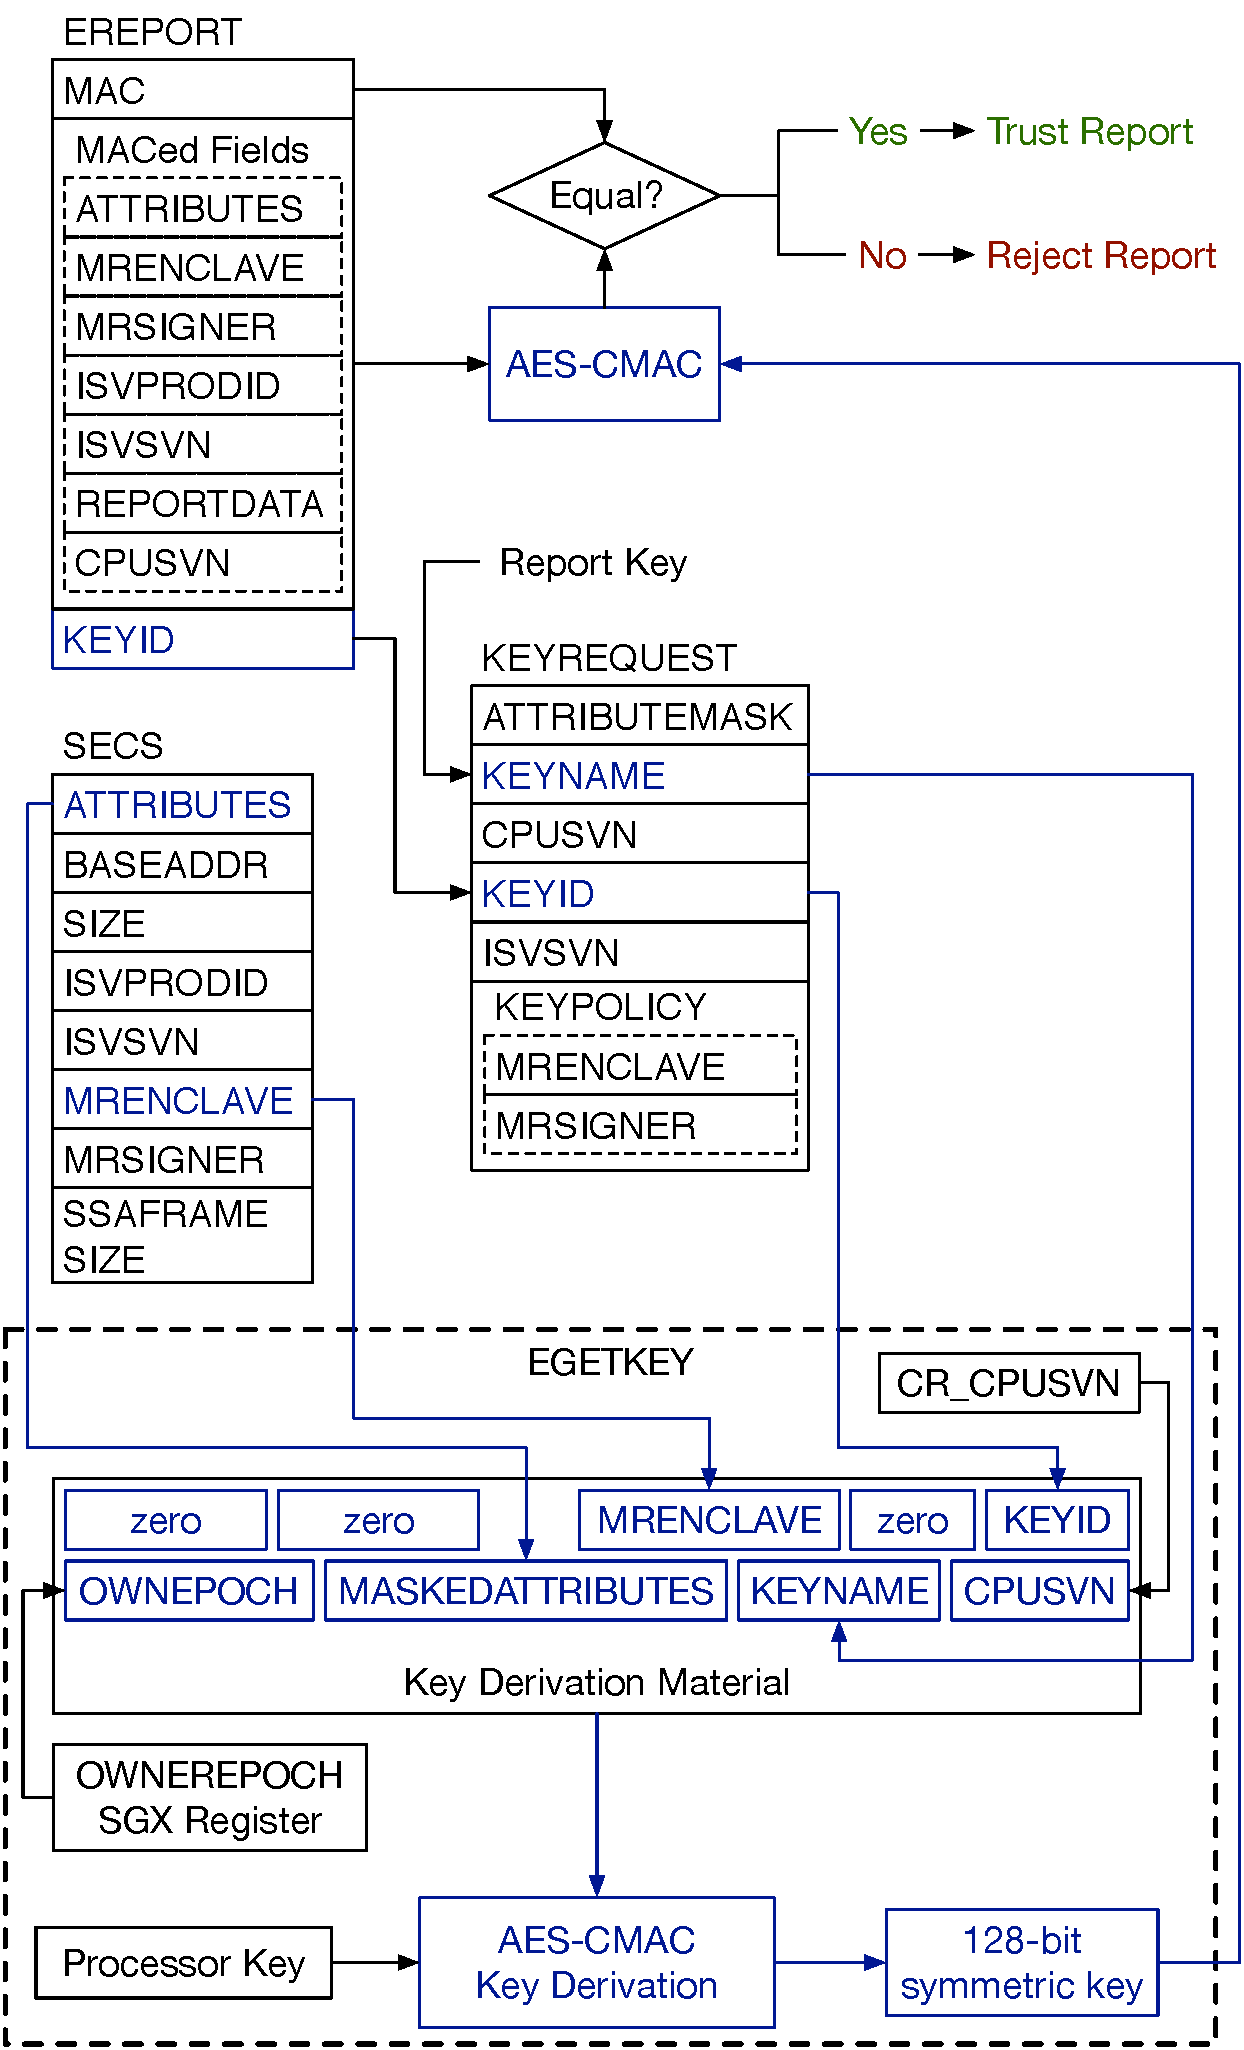
\includegraphics[width=87mm]{figures/sgx_ereport_check.pdf}
  \caption{
    The authenticty of the REPORT structure created by \texttt{EREPORT} can and
    should be verified by the report's target enclave. The target's code uses
    \texttt{EGETKEY} to obtain the key used for the MAC tag embedded in the
    REPORT structure, and then verifies the tag.
  }
  \label{fig:sgx_ereport_check}
\end{figure}

The report key returned by \texttt{EGETKEY} is derived from a secret embedded
in the processor~(\S~\ref{sec:sgx_egetkey}), and the key material includes the
target enclave's measurement. The target enclave can be assured that the MAC
tag in the report was produced by the SGX implementation, for the following
reasons. The cryptographic properties of the underlying key derivation and
MAC algorithms ensure that only the SGX implementation can produce the MAC tag,
as it is the only entity who can access the processor's secret, and it would be
impossible for an attacker to derive the report key without knowing the
processor's secret. The SGX design guarantees that key produced by
\texttt{EGETKEY} depends on the calling enclave's measurement, so only the
target enclave can obtain the key used to produce the MAC tag in the report.

\texttt{EREPORT} uses the same key derivation process as \texttt{EGETKEY}
does when invoked with KEYNAME set to the value that represents a Report Key.
For this reason, \texttt{EREPORT} requires the virtual address of a
\textit{Report Target Info}~(TARGETINFO) structure that contains the
measurement-based identity and attributes of the target enclave.

% EGETKEY: SDM S 41.4.1
% Key Derivation: SDM Table 41-43

When deriving a report key, \texttt{EGETKEY} behaves slightly differently than
it does in the case of seal keys, as shown in
Figure~\ref{fig:sgx_ereport_check}. The key generation material never includes
the fields corresponding to the enclave's certificate-based identity
(MRSIGNER, ISVPRODID, ISVSVN), and the KEYPOLICY field in the KEYREQUEST
structure is ignored. Furthermore, the SGX implementation SVN~(CPUSVN) value
used for key generation is determined by the current CPUSVN, instead from being
read from the Key Request structure.


Last, \texttt{EREPORT} sets the KEYID field in the key generation material to
the contents of an SGX configuration register (CR\_REPORT\_KEYID) that is
initialized with a random value when SGX is initialized. The KEYID value is
also saved in the attestation report, but it is not covered by the MAC tag.


\subsubsection{Enclave Approval}
\label{sec:sgx_launch_enclave}

% ATTRIBUTES: SDM S 38.7.1
% EINIT: SDM S 41.3
% EINITTOKENKEY is bit 5, INTEL_ONLY_MASK is 0x20

Instead of implementing potentially complex access checks

% EINIT Token Structure (EINITTOKEN): SDM S 38.14

\begin{figure}[hbt]
  \centering
  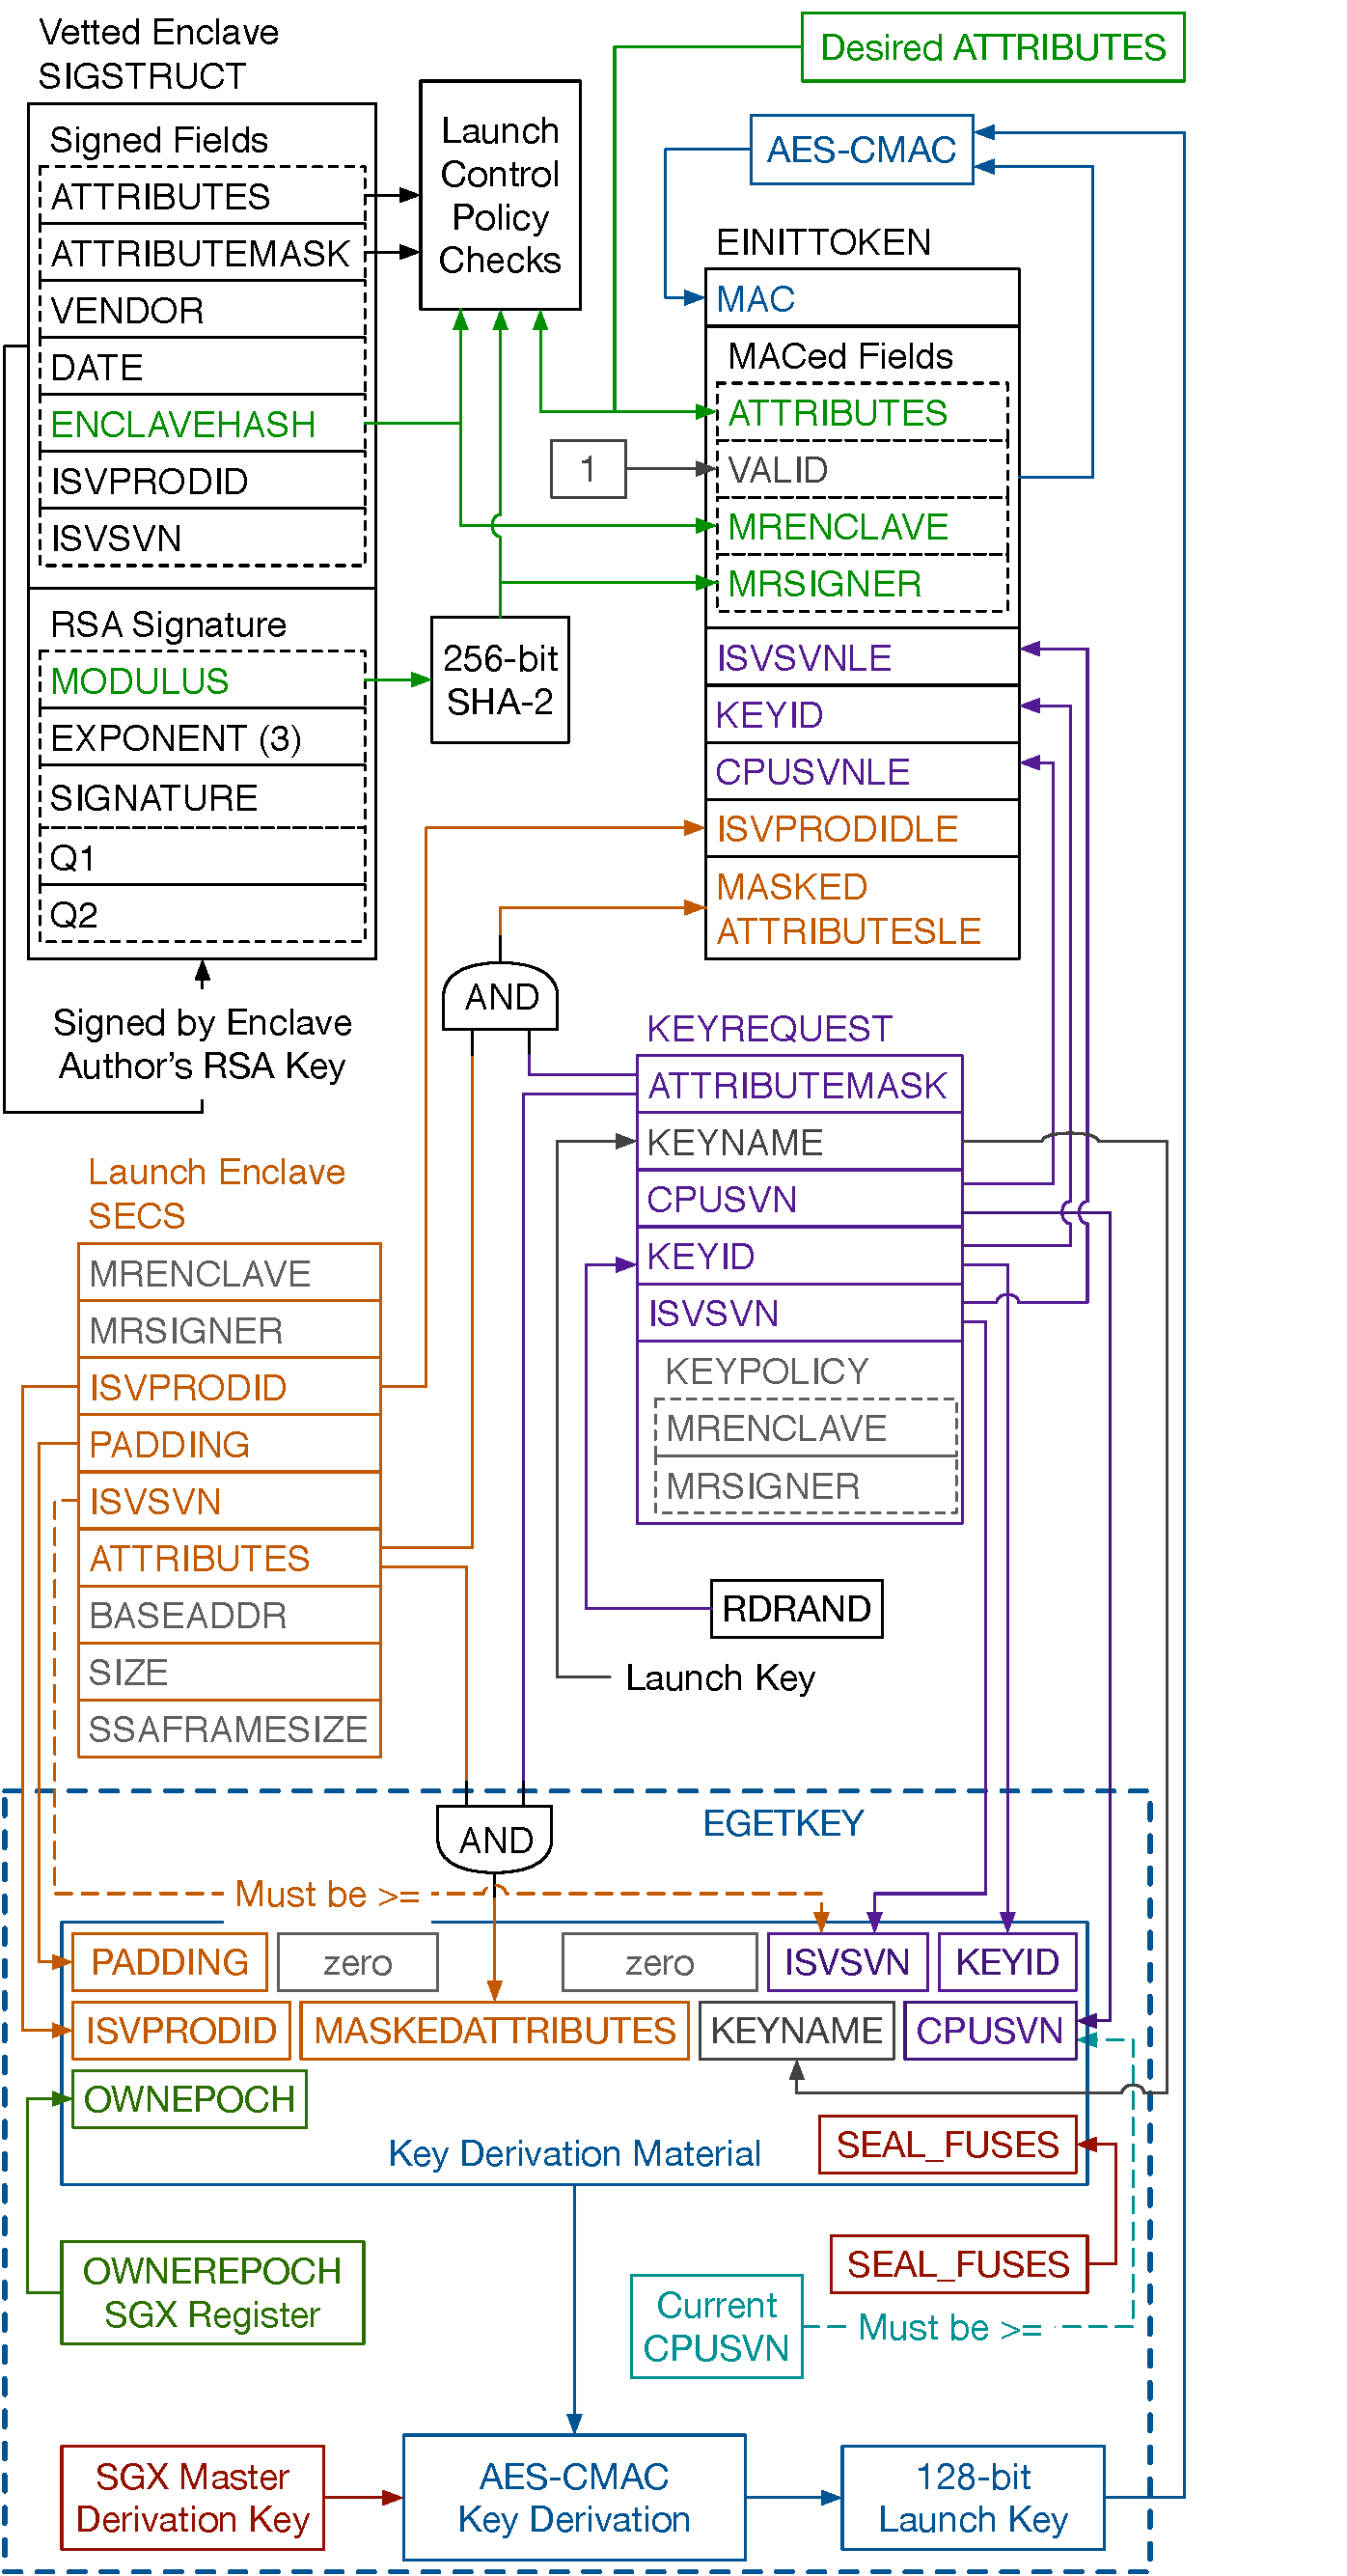
\includegraphics[width=87mm]{figures/sgx_einittoken.pdf}
  \caption{
    The SGX Launch Enclave computes the EINITTOKEN.
  }
  \label{fig:sgx_einittoken}
\end{figure}



% MRSIGNER: SDM S 39.4.1.2

After an enclave gets cleared by the SGX Launch Enclave and is initialized via
\texttt{EINIT}, it can authenticate itself to a remote party by participating
in a software attestation process.


\subsubsection{The Quoting Enclave}
\label{sec:sgx_quoting_enclave}

While the SDM paints a complete picture of the local attestation mechanism, it
is a lot more secretive about the Quoting Enclave and the underlying keys.
Fortunately, the SGX patents~\cite{intel2013patent1, intel2013patent2} shed
some light on the topic.



\subsubsection{Licensing}
\label{sec:sgx_licensing}

However, the software attestation scheme in SGX's design, summarized in
Figure~\ref{fig:sgx_attestation_overview} is unnecessarily complicated by the
decision to deeply couple software attestation with
\textbf{an enclave licensing mechanism that allows Intel to force itself as an
intermediary in the distribution of all enclave software}.
